\section{Esempio di funzionamento}

In questo esempio di funzionamento si utilizzerà il gene ENSG00000280145, situato nel cromosoma 21 dell'uomo sapiens (GRCh38 / hg38). E' stato prima scaricato il   genoma di riferimento da ensembl in formato fasta e la relativa annotazione in formato gtf. Dal file gtf (contenente l'annotazione per l'intero genoma) è stata isolata l'annotazione relativa al gene ENSG00000280145.

\subsection{Generazione delle read con Flux Simuator}

Si è scelto di utilizzare Flux Simulator per la generazione delle read paired-end. Il suo utilizzo non è particolarmente complicato, ma è necessario passare i diversi parametri attraverso un file con estensione .p. Il file utilizzato in questa simulazione è il seguente:

\begin{figure}[h]
	\centering
	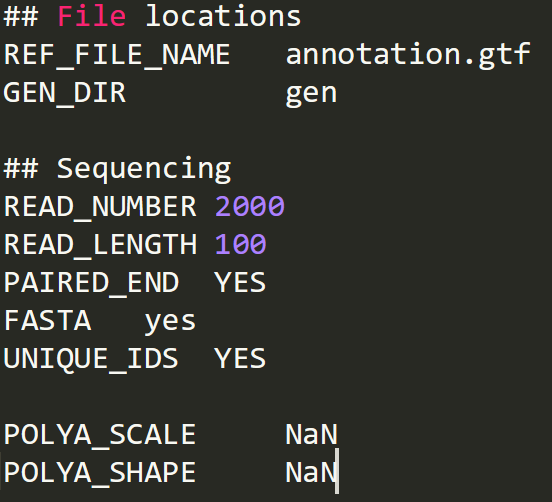
\includegraphics[height=7cm,width=10cm]{images/parameters2.png}
  \caption{Il file contente i parametri di Flux Simulator}
  \label{fig:Parameters}
\end{figure}

Vengono così generati due file contenti 2000 read di lunghezza 100, in formato fasta, che saranno dati in input ad ASGAL.

\newpage

\subsection{Utilizzo di ASGAL}

ASGAL viene eseguito via linea di comando, richiamando lo script principale usando come parametri:

\begin{itemize}
	\item Il \textbf{genoma} di riferimento (opzione \textbf{-g})
	\item L'\textbf{annotazione} del genoma (opzione \textbf{-a})
	\item I due file contenti \textbf{read} (opzioni \textbf{-s} e \textbf{-s2})
	\item La \textbf{cartella di destinazione} dell'output (opzione \textbf{-o})
	\item L'indicazione delle \textbf{read paired-end} (opzione \textbf{--paired})
	\item La \textbf{fragment library type} (opzione \textbf{-f}), opzionale per velocizzare la fase di allineamento
\end{itemize}

Questo script richiama nell'ordine lo Splice-Aware Aligner, il Formattatore SAM e il Rilevatore di eventi di Alternative Splicing, visualizzando alcune informazioni sul funzionamento.

Questa immagine mostra il funzionamento di ASGAL:

\begin{figure}[h]
	\centering
	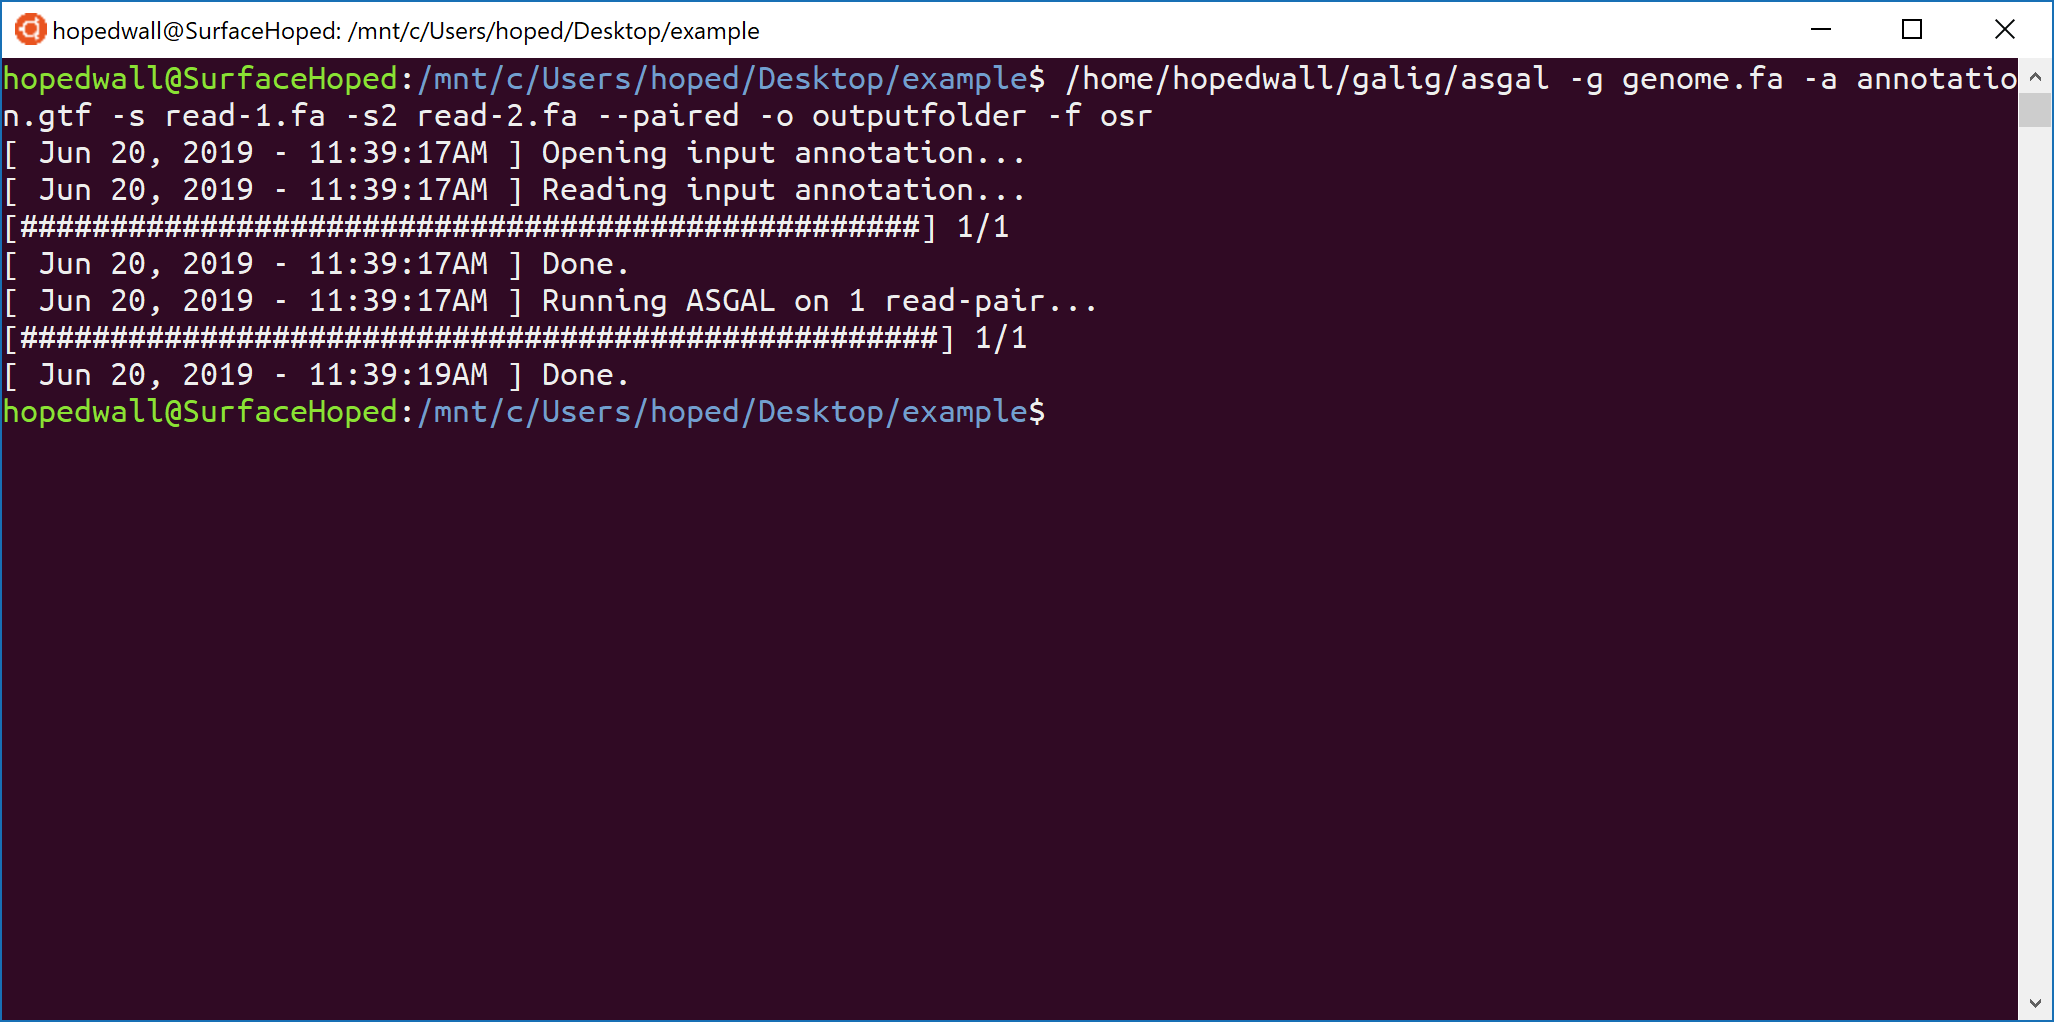
\includegraphics[width=\linewidth]{images/prompt.png}
  \caption{ASGAL in funzione}
  \label{fig:ASGALPrompt}
\end{figure}

Sebbene sia possibile eseguire ciascuno script singolarmente, si raccomanda di usare lo script principale per un utilizzo più immediato. 

\newpage

\subsection{Risultati}

Dall'esecuzione vengono prodotti i seguenti file:

\begin{figure}[h!]
	\centering
	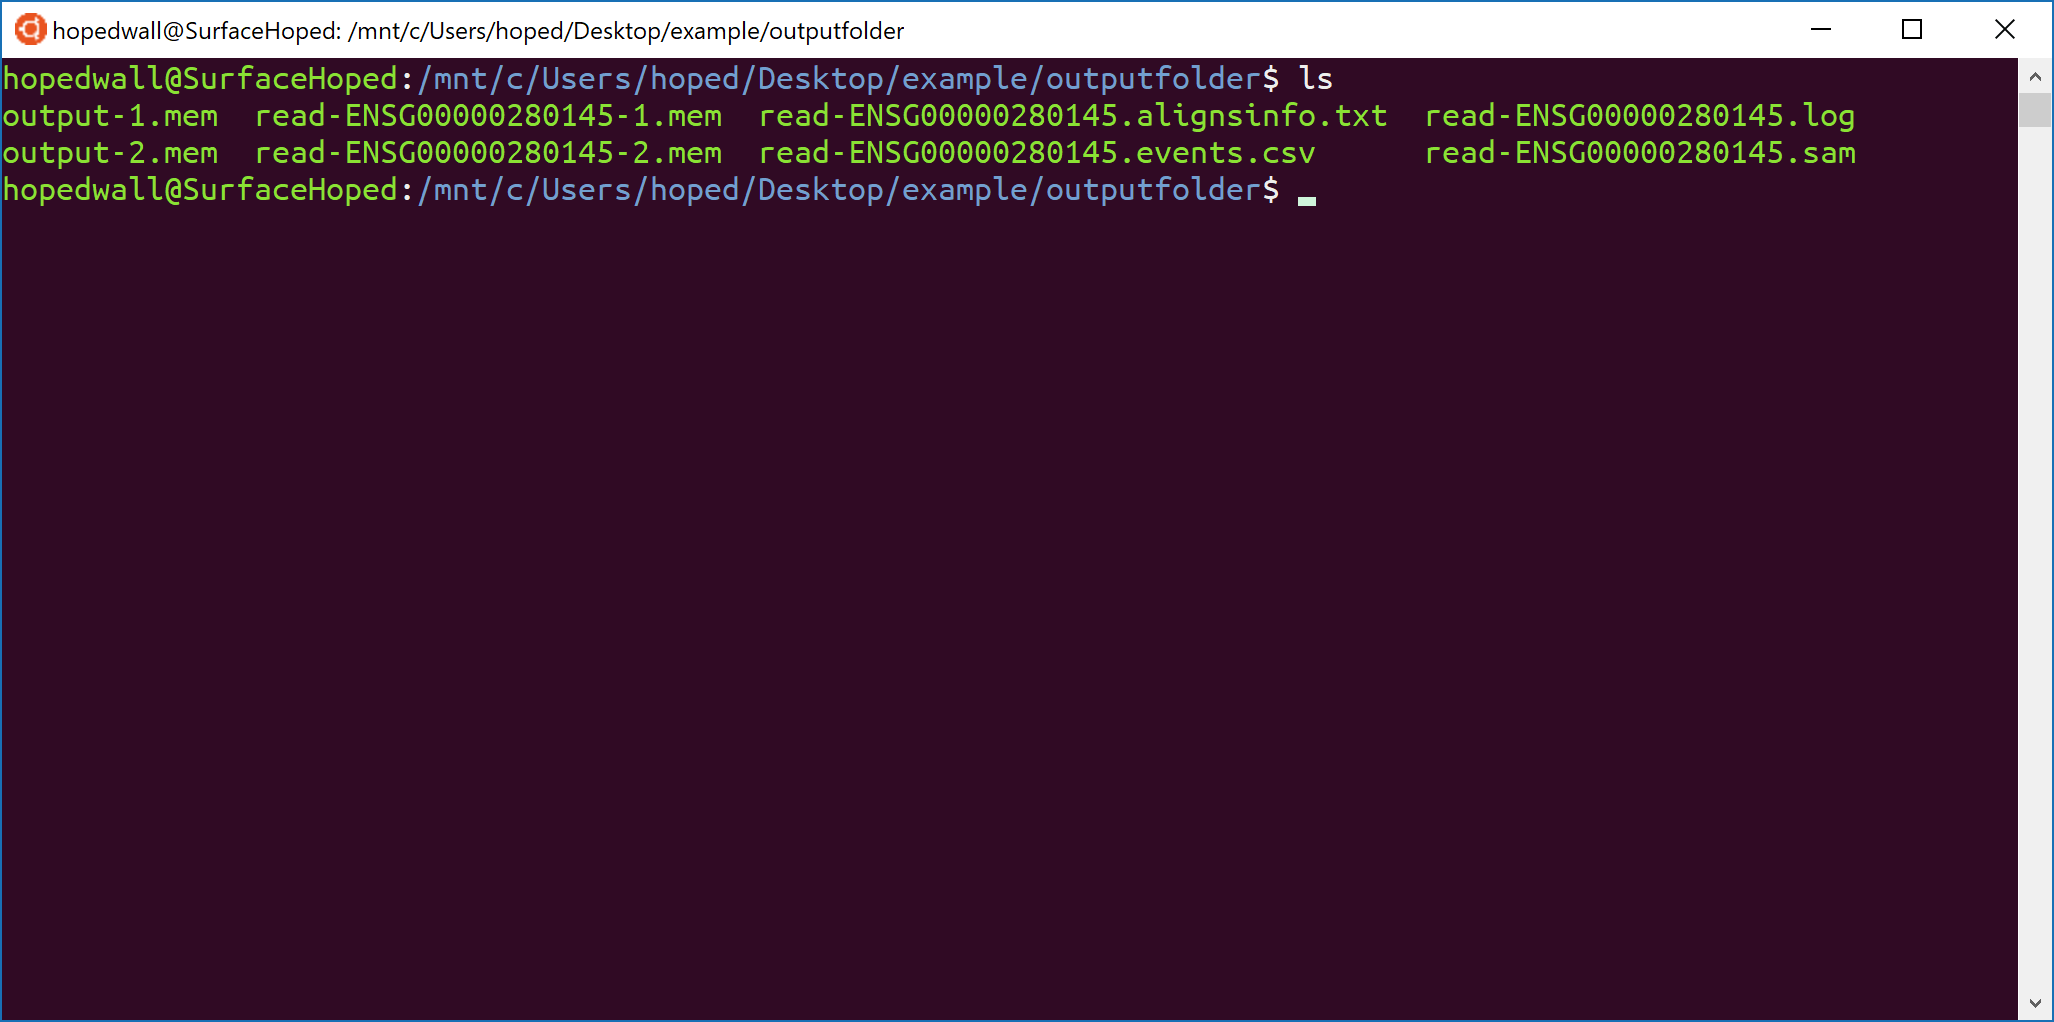
\includegraphics[width=\linewidth,height=1.25cm]{images/fileprodotti.png}
  \label{fig:ProducedFiles}
\end{figure}

Ovvero:

\begin{itemize}
	\item I file .mem prodotti dal primo step
	\item Il file .sam e .alignsinfo.txt prodotti dal secondo step
	\item	Il file .events.csv prodotti prodotto dal terzo step
\end{itemize}

Analizzando il file alignsinfo.txt si nota che oltre il 98\% delle read sono state mappate.

\begin{figure}[h!]
	\centering
	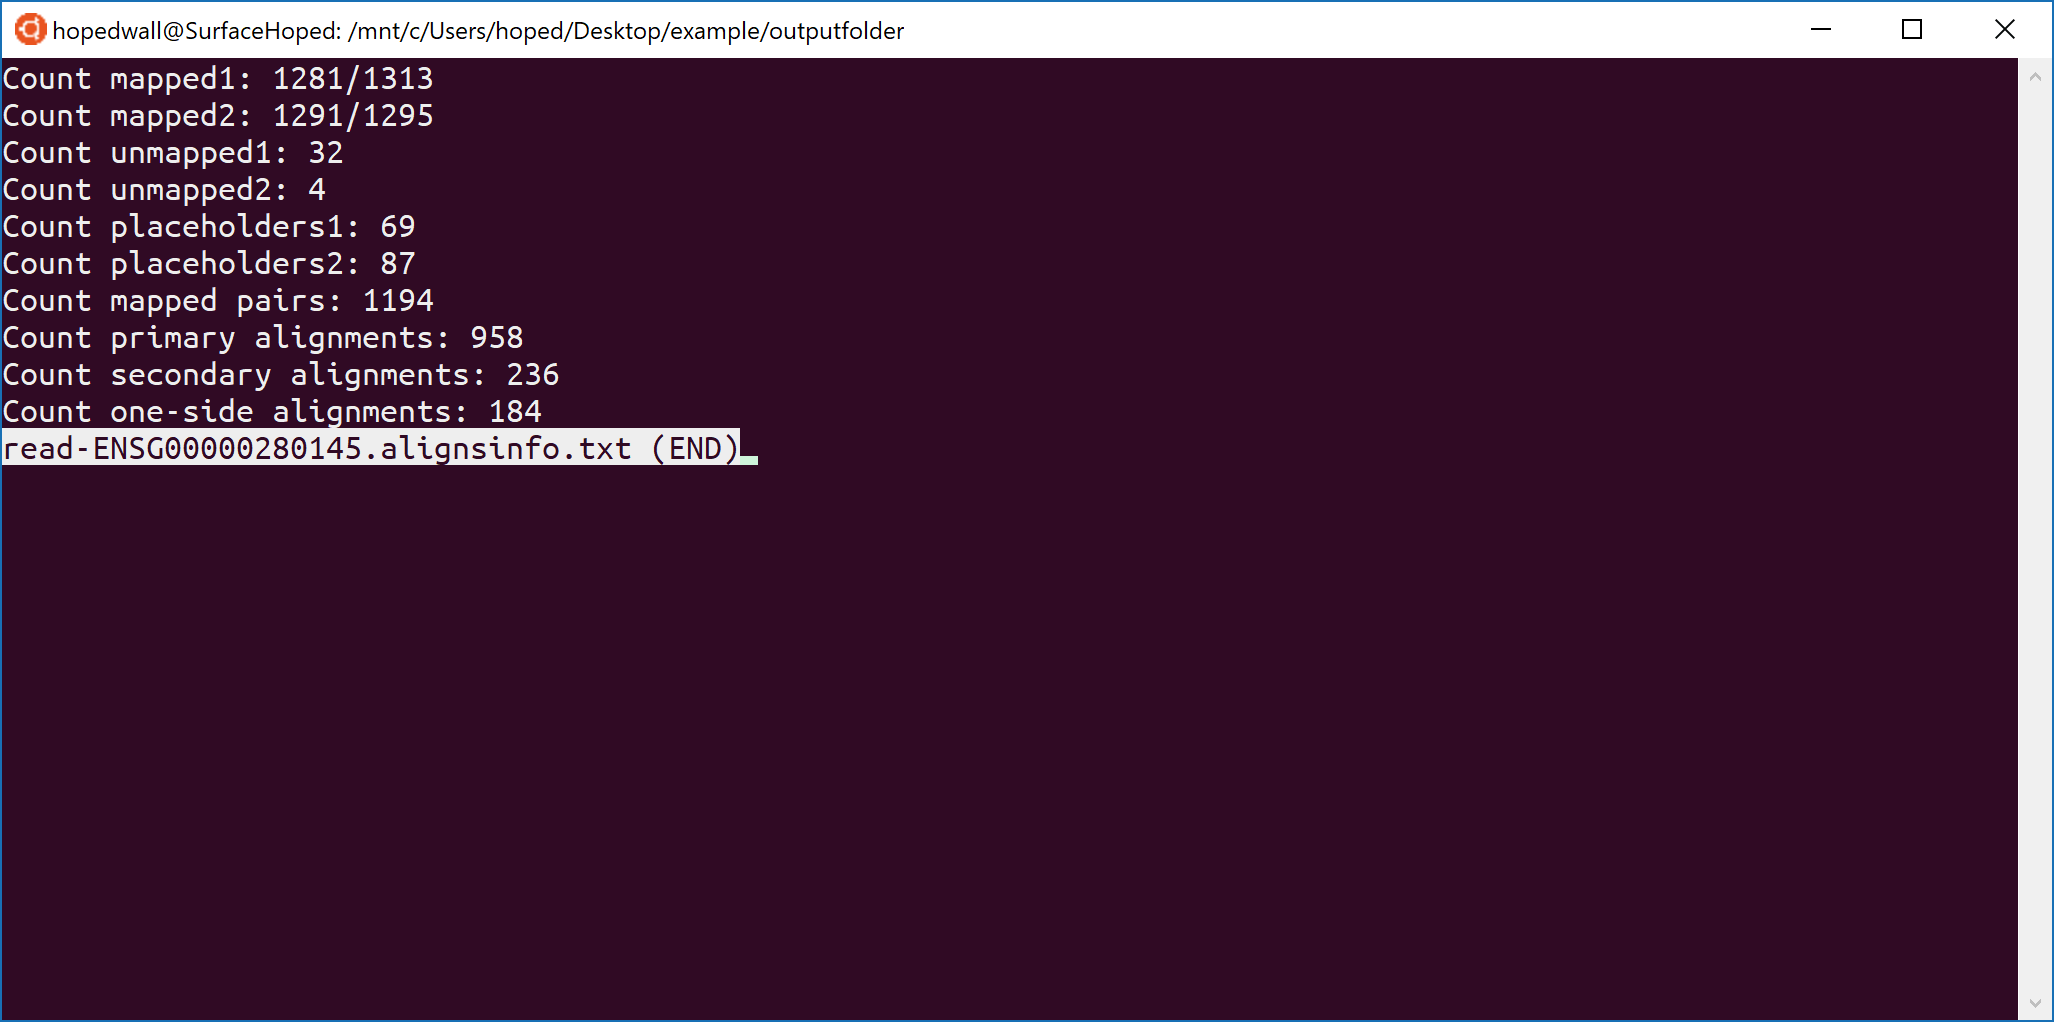
\includegraphics[width=\linewidth,height=10cm]{images/alignsinfotxt.png}
  \label{fig:AlignsInfoExperiment}
\end{figure}

\newpage

Il file .events.csv contiene gli eventi di Alternative Splicing rilevati da ASGAL:

%\begin{itemize}
%	\item la prima colonna rappresenta il \textbf{tipo di evento}
%	\item la seconda colonna rappresenta la \textbf{posizione di inizio} nella genomica
%	\item	la terza colonna rappresenta la \textbf{posizione di fine} nella genomica
%	\item la quarta colonna rappresenta il \textbf{numero di read} che suggeriscono l'evento
%	\item la quinta colonna rappresenta il/i \textbf{nomi dei trascritti} che suggeriscono l'evento
%\end{itemize}

\begin{figure}[h!]
	\centering
	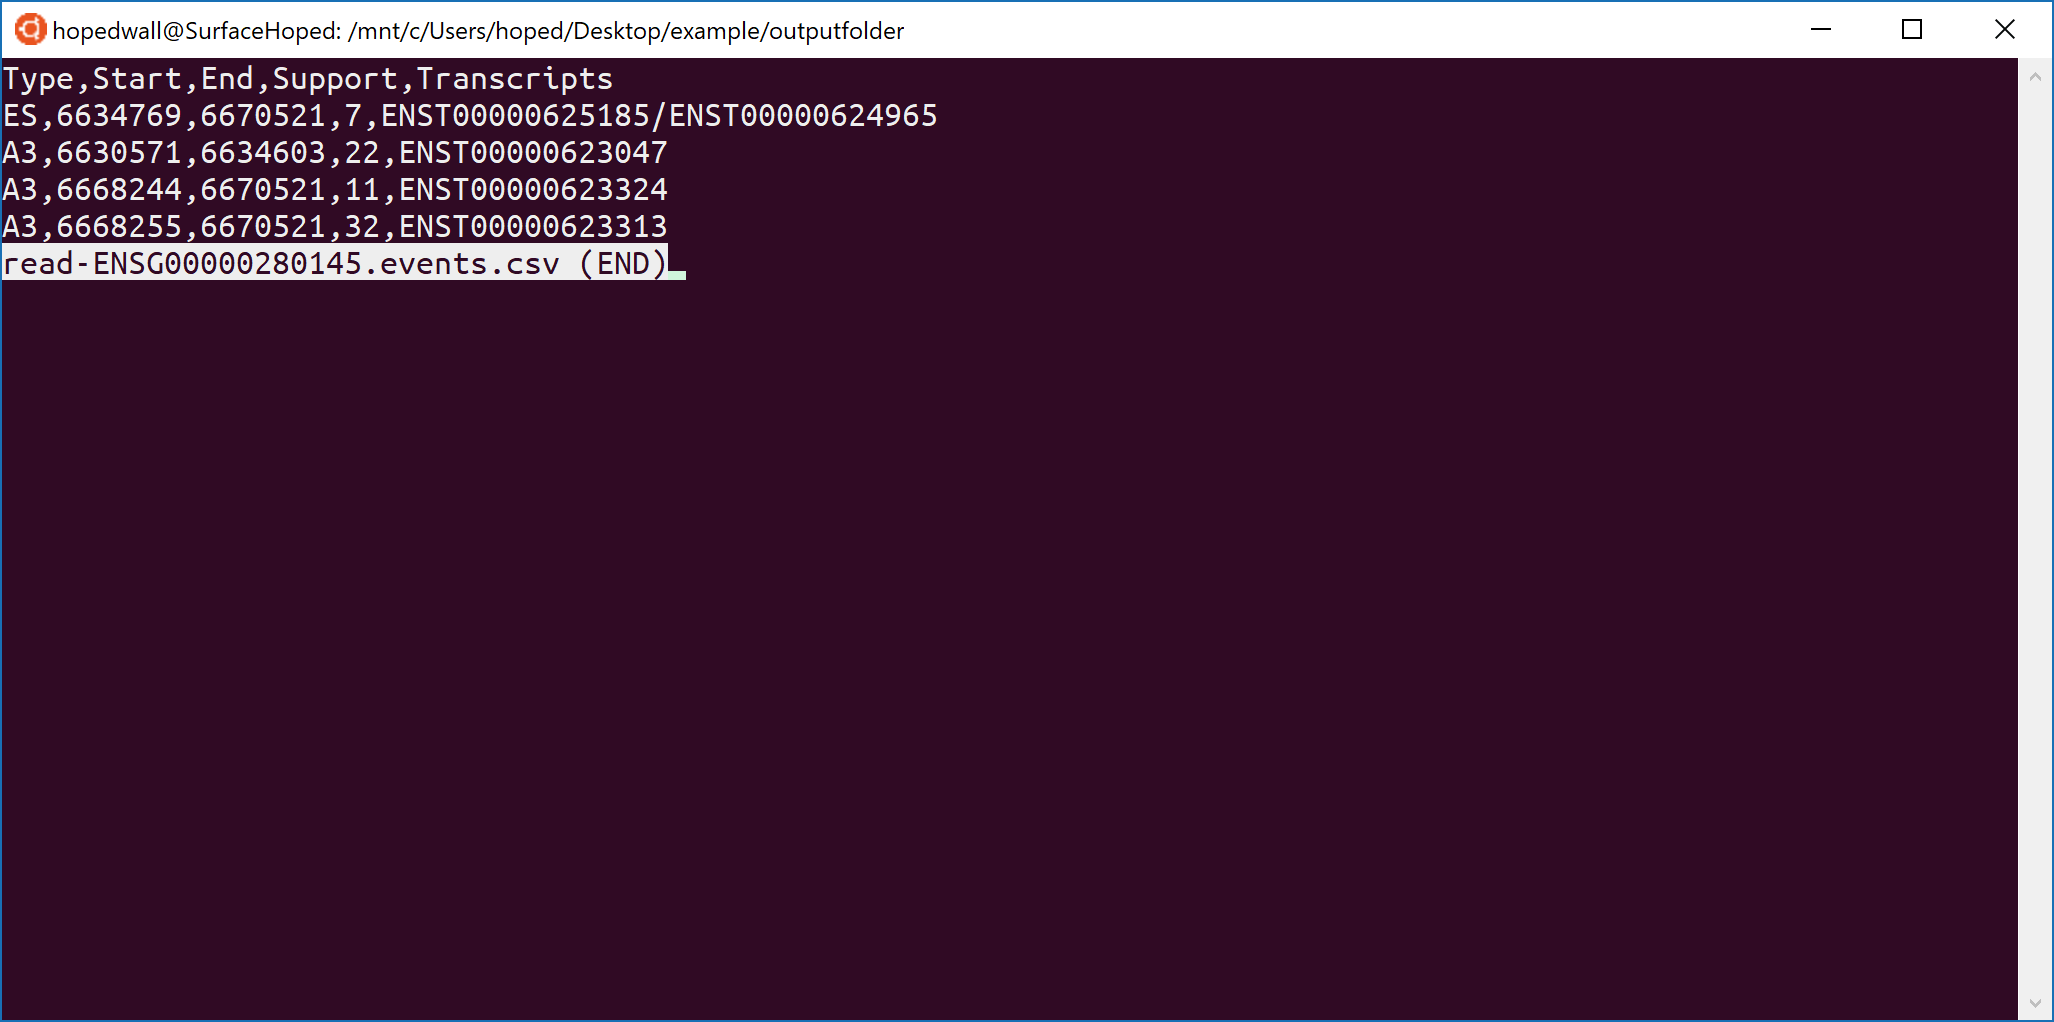
\includegraphics[width=\linewidth]{images/results.png}
  \label{fig:Parameters}
\end{figure}

Sono stati rilevati tre eventi di Alternative Donor Site e un evento di Exon Skipping.

\newpage